\subsubsection{UC4 - Impostazione dei parametri di personalizzazione}
\begin{figure}[h]
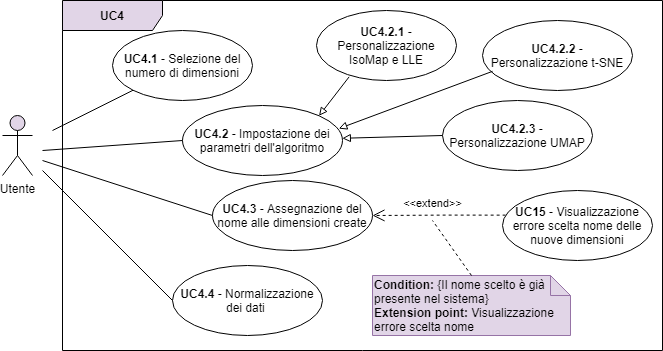
\includegraphics[width=\linewidth]{section/Images/UC4.png}
\centering
\caption{UC4 - Impostazione dei parametri di personalizzazione}
\end{figure}
\begin{itemize}
	\item \textbf{Attore primario}: Utente.
	\item \textbf{Precondizioni}: L'utente ha caricato dei dati nel sistema [UC1], ha scelto le dimensioni da utilizzare [UC2] e ha scelto la visualizzazione che desidera vedere [UC3].
	\item \textbf{Postcondizioni}: Viene aggiornata la visualizzazione scelta con i nuovi parametri impostati dall'utente.
	\item \textbf{Scenario principale}:
		\begin{enumerate}
			\item Viene presentata all'utente una sezione per apportare delle modifiche ai parametri relativi alla visualizzazione scelta;
			\item L'utente decide le dimensioni da visualizzare e le altre funzionalità specifiche del grafico. Se queste non dovessero essere modificate, verranno applicati valori di default tipici per ogni visualizzazione;
			\item Al termine, l'utente dovrà premere sul pulsante per la conferma e l'invio delle nuove preferenze.
		\end{enumerate}
\end{itemize}